% !TeX root=SBUKThesis-main.tex
\clearpage
\thispagestyle{empty}
\chapter{روش‌های پیشنهادی}\label{chap3}

\section{مقدمه}
همانطور که گفته شد، 
عملکرد مدل‌های زبانی بزرگ به‌شدت به مهندسی اعلان وابسته است، چرا که دستورات به‌طور مستقیم بر تفسیر مدل از وظایف و همچنین نحوه تولید خروجی تاثیر می\/گذارند. 
بنابراین، دستورات نقش حیاتی در اثربخشی مدل‌های زبانی بزرگ ایفا می‌کنند، فرآیندی که معمولاً از طریق آنچه به‌عنوان مهندسی دستور شناخته می‌شود، بهینه‌سازی می‌گردد.
استراتژی‌های پرکاربردی مانند
 زنجیره تفکر \cite{CoT} 
اثربخشی خود را در بهبود توانمندی‌های استدلالی مدل‌های زبانی با تجزیه مسائل پیچیده به گام‌های میانی نشان داده‌اند
\cite{selfconsistencyimproveschainthought}, \cite{TowardsUnderstandingCoTPrompting}, \cite{cotcollectionimprovingzeroshot}, \cite{revealingmysterychainthought}.
با این حال، استراتژی‌های دستی طراحی‌شده توسط انسان، به دلیل وابستگی به شهود انسانی، غالباً برای وظایف خاص دامنه محور، بهینه نبوده و نمی‌توانند به‌طور کامل از ظرفیت مدل‌های پایه بهره‌برداری کنند.
از سوی دیگر، با پیشرفت مداوم مدل‌های زبانی و تغییر قابلیت‌های آن‌ها، مؤثرترین دستورات نیز ممکن است دستخوش تغییر شوند.
به‌طور کلی، مهندسی اعلان که به‌صورت دستی انجام می‌شود، فرآیندی زمان‌بر بوده و نتایجی کمتر از حد بهینه به همراه دارد.
این محدودیت‌ها موجب شده است که تولید خودکار دستورات به‌عنوان یک حوزهٔ تحقیقاتی مهم در هوش مصنوعی مطرح گردد 
\cite{textpatternseffectivechain}, \cite{APE}.
همانطور که در فصل قبل دیدیم، الگوریتم‌های مختلفی برای بهینه‌سازی دستورات معرفی شده‌اند؛ از جمله
 بهینه\/سازی با اعلان \cite{opro}، مولد اعلان \cite{PromptBreeder} و سایر روش ها \cite{ExploringthePromptSpaceofLLMsthroughEvolutionarySampling}  \cite{epiccosteffectivesearchbasedprompt}.
در این میان، روش مولد اعلان با استفاده از یک چارچوب تکاملی و خودارجاعی، از طریق تکرار فرآیند جهش و ارزیابی یک جمعیت از دستورات وظیفه، به بهینه‌سازی دستورات می‌پردازد.
اگرچه نشان داده شده است که روش مود اعلان برای وظایف استدلالی و طبقه‌بندی مؤثر است، اما پیچیدگی طراحی آن موجب کاهش قابلیت تعمیم این روش می‌شود. افزون بر این، عدم تنوع کافی در دستورات تولید شده می‌تواند چالش‌زا باشد.
وابستگی به چندین لایه بهینه‌سازی، سازوکارهای خودارجاعی و حتی به‌کارگیری تکنیک‌هایی برای فریب مدل زبانی
\footnote{صفحه ۷ مقاله مولد اعلان : «توجه داشته باشید که ما به مدل زبانی ‘دروغ’ گفته‌ایم و بیان کرده‌ایم که ترتیب نزولی است.»}
 ممکن است موجب عدم موفقیت این روش هنگام به‌کارگیری بر روی مدل‌های زبانی جدید شود.

در این مطالعه، جایگزینی ساده‌تر و شفاف‌تر برای مولد اعلان تحت عنوان مولد اعلان ساده
\LTRfootnote{SimplePromptBreeder}
 پیشنهاد می‌شود که ضمن حفظ نقاط قوت اصلی، کاستی‌های آن را نیز برطرف می‌سازد.
با ساده‌سازی چارچوب تکاملی بهینه‌سازی دستورات، روش پیشنهادی، ضمن کاهش پیچیدگی، قابلیت تفسیر و مقیاس‌پذیری را نیز بهبود می‌بخشد (همان‌طور که در شکل~\ref{fig_teaser} نشان داده شده است).
این رویکرد در تلاش است تا تولید خودکار دستورات را کاربردی‌تر و در دسترس‌تر سازد.

 \begin{figure}[!t]
	\centering
	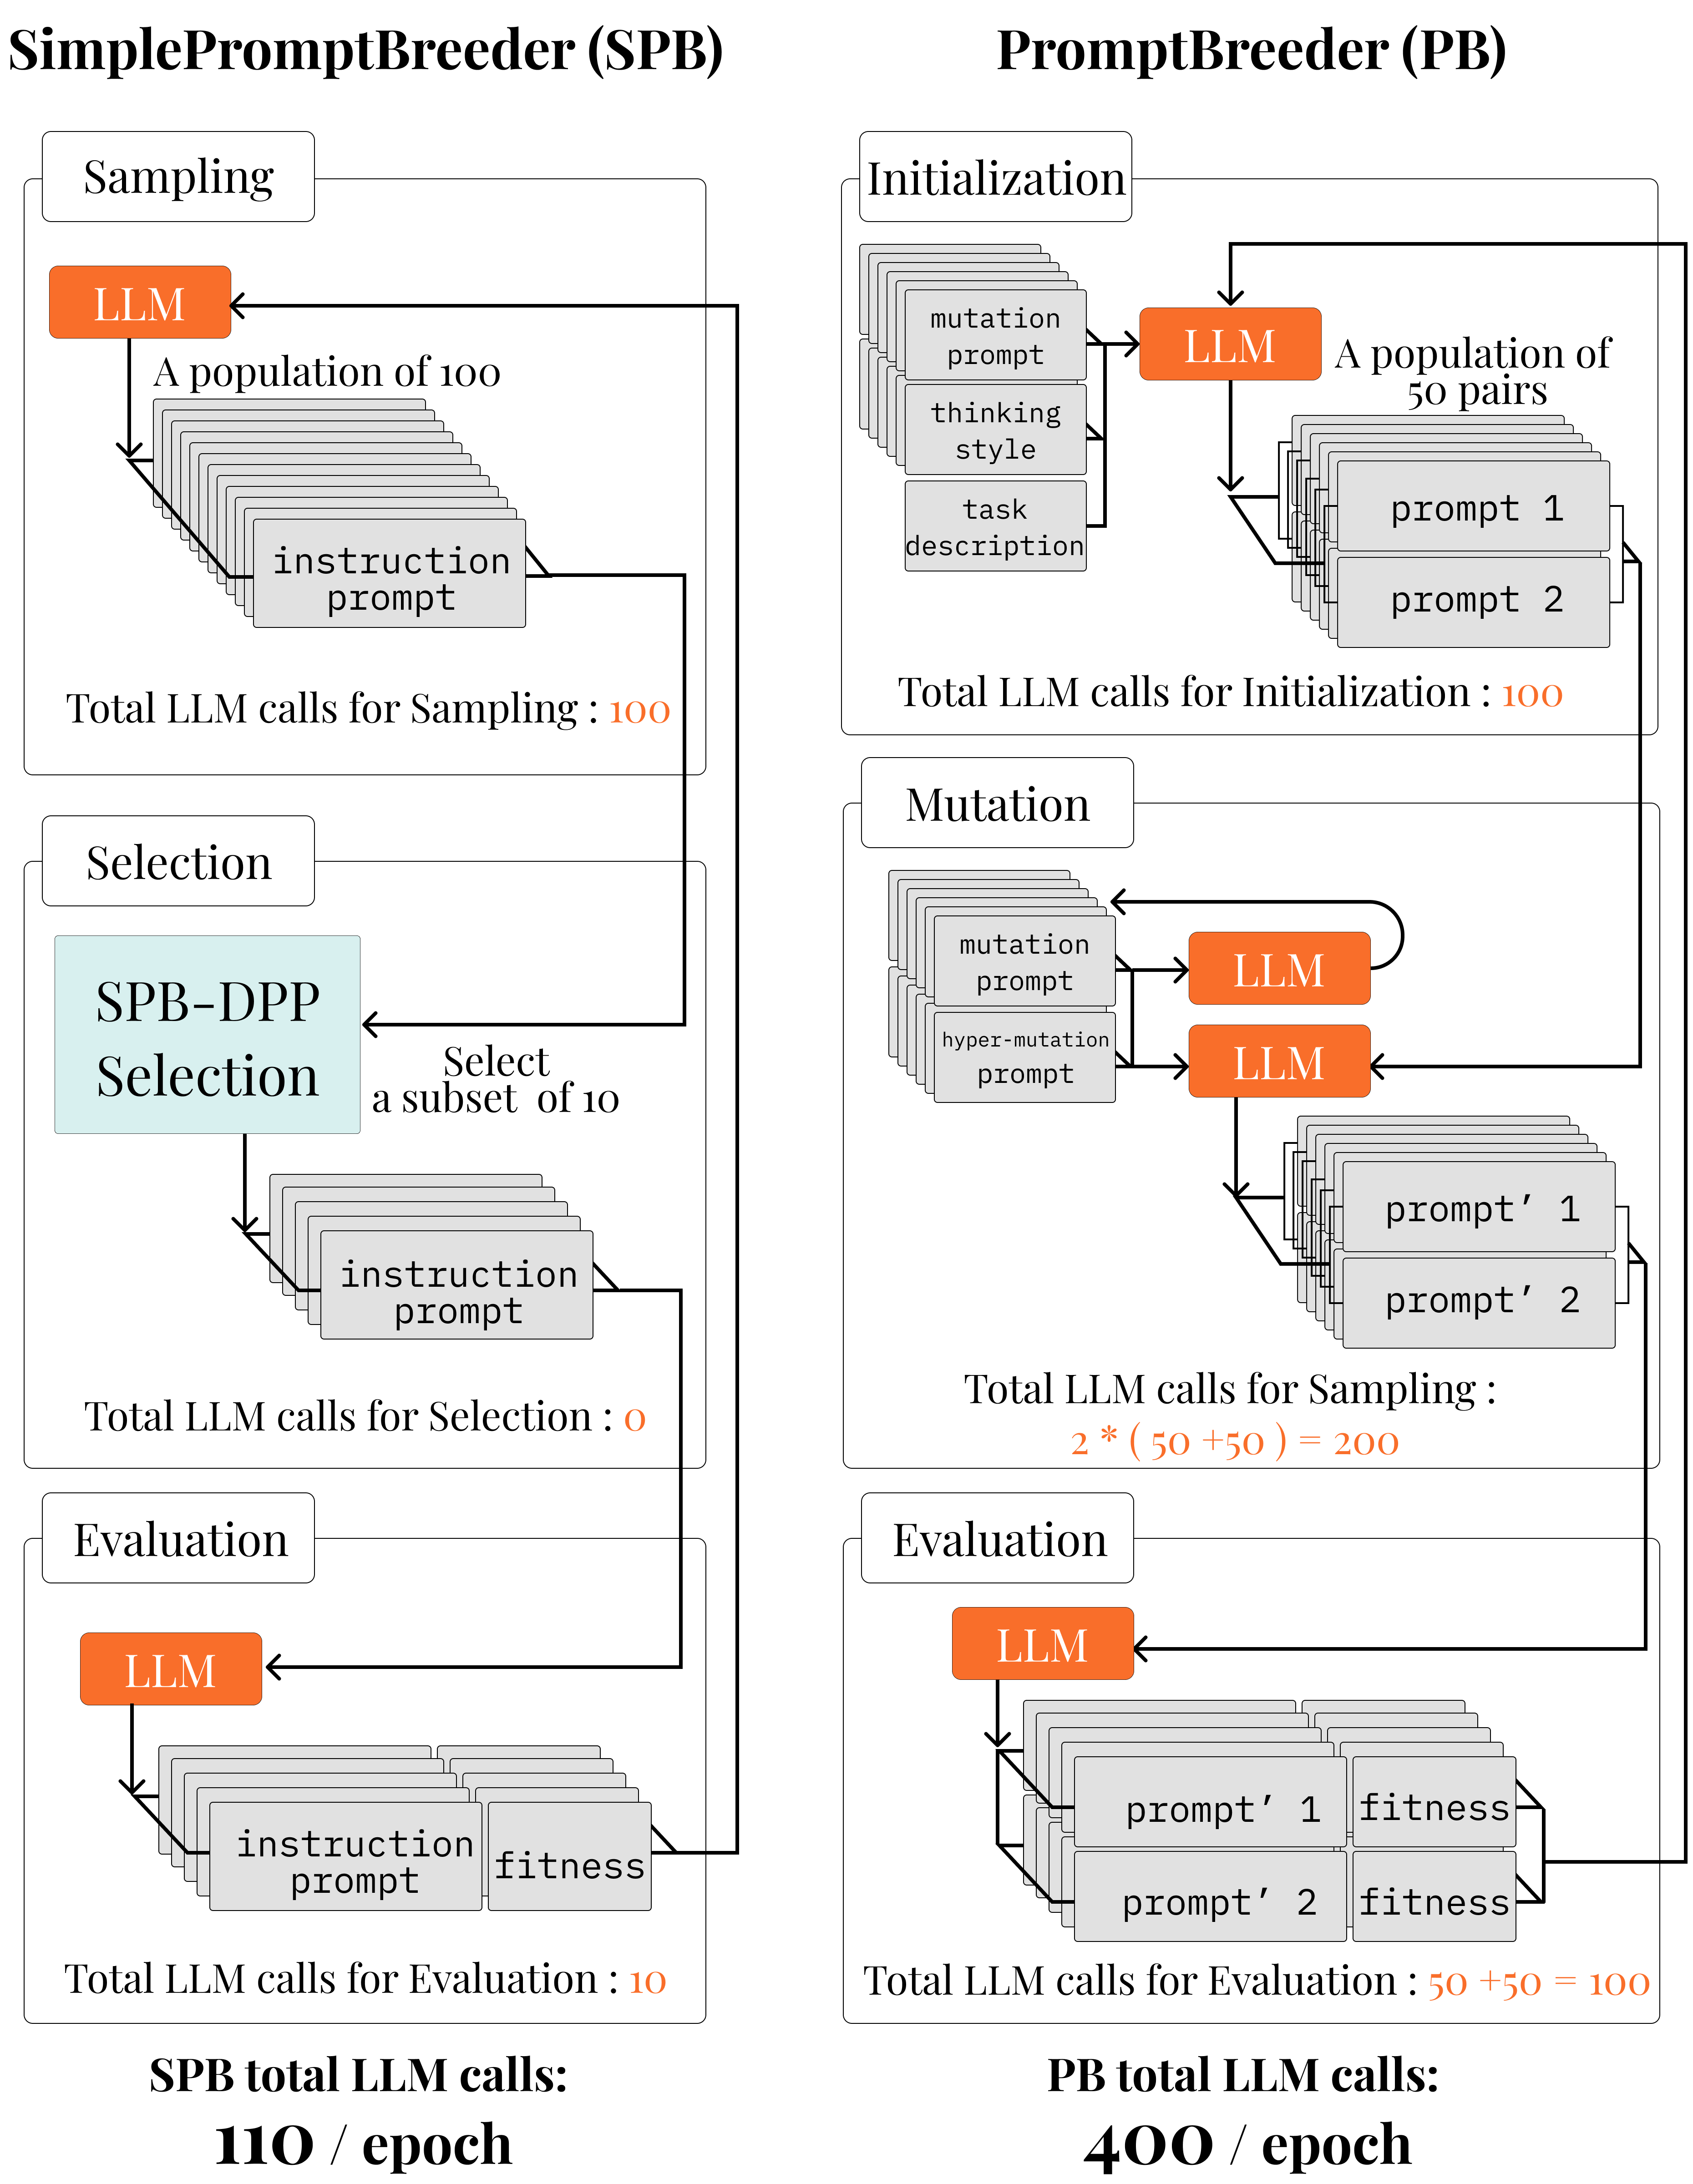
\includegraphics[width=100mm]{images/tf}
	\caption{مقایسه پیچیدگی محاسباتی روش مولد اعلان و روش مولد اعلان ساده}
	\label{fig_teaser}
\end{figure}

مولد اعلان ساده به‌صورت تکرارشونده دستورات را بررسی می‌کند و با بهره‌گیری مستقیم از یک مدل احتمالاتی به نام فرآیندهای نقطه\/ای دترمینانی، به بهینه‌سازی تنوع و کیفیت آن‌ها می‌پردازد. مدل های احتمالی فرآیندهای نقطه\/ای دترمینانی، به‌گونه‌ای طراحی شده‌اند که راهکارهای بهینه‌ای برای مسئله انتخاب در فضای دستورات ارائه دهند به گونه\/ای که هم با کیفیت و هم متنوع باشند.
 
فرضیهٔ تحقیق ما این است که استفاده از فرآیندهای نقطه\/ای دترمینانی می‌تواند تعداد دفعات فراخوانی مدل زبانی بزرگ را برای یافتن دستورات بهینه کاهش داده و در عین حال، سطح عملکرد رقابتی را حفظ نماید.
سادگی و ظرافت ریاضی این رویکرد همچنین می‌تواند موجب افزایش استحکام آن در برابر انواع مدل‌های زبانی شود که این روش بر روی آن‌ها اعمال می‌گردد.
از طرفی  ساختار ریاضی این روش، آن را به جایگزینی عملی و قابل تفسیر برای روش‌های پیچیده تبدیل می‌کند.




\section{روش مولد اعلان ساده}

برای استفاده از مدل‌های زبانی بزرگ با دستورالعمل
\LTRfootnote{instructed LLMs}
 مانند Mistral \cite{mistral}، لازم است اعلان‌ها در قالب خاصی سازمان‌دهی شوند تا حالت مکالمه‌ای
 \LTRfootnote{chat-mode}
  شبیه‌سازی شود.  
این قالب بر پایه‌ی ساختار کلید-مقدار
\LTRfootnote{key-value}
 استوار است، که در آن هر کلید، نقش
 \LTRfootnote{role}
  را مشخص می‌کند و مقدار متناظر، محتوا یا پیام مربوط به آن نقش را شامل می‌شود. سه نقش رایج در این قالب وجود دارد: سیستم، دستیار و کاربر. برای نقش سیستم، محتوا به عنوان دستورالعمل‌هایی برای مدل زبانی عمل می‌کند تا وظایف مشخصی را انجام داده و به اعلان‌های کاربر پاسخ دهد.  
این دستورالعمل‌ها با عنوان اعلان دستوری
\LTRfootnote{instruction prompt}
 شناخته می‌شوند و تأثیر بسزایی بر کیفیت پاسخ‌های تولید شده توسط مدل دارند.

برای کشف این نوع اعلان‌های دستوری، از یک الگوریتم تکاملی استفاده می‌کند که به طور کارآمد یک جستجوی محلی
\LTRfootnote{Local Search}
 را در فضای بی‌نهایت اعلان‌ها انجام می‌دهد.  
 \begin{figure}[!t]
 	\centering
 	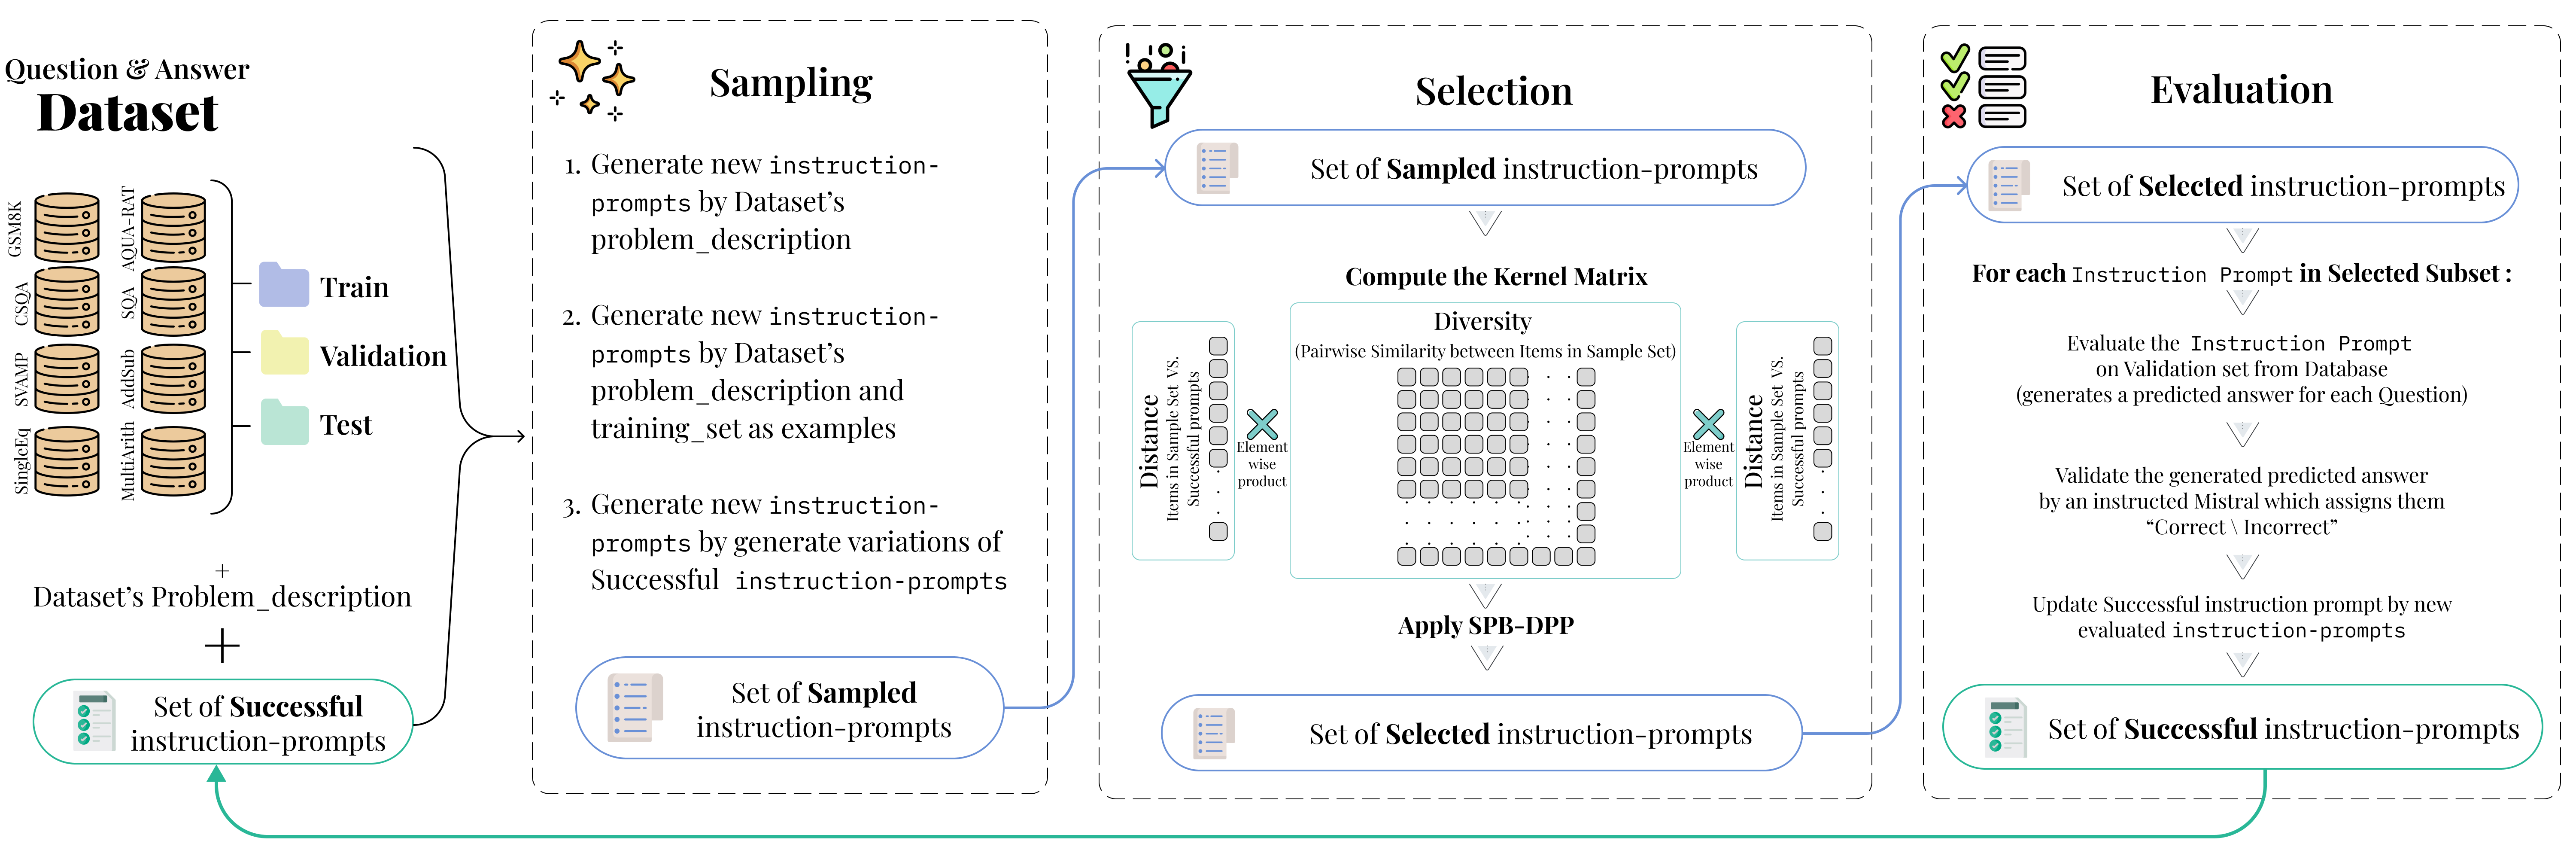
\includegraphics[width=140mm]{images/flow}
 	\caption{دیاگرام روش مولد اعلان ساده}
 	\label{fig_flowchart}
 \end{figure}

 
همان‌طور که در شکل \ref{fig_flowchart} نشان داده شده است، مولد اعلان ساده یک چرخه سه مرحله‌ای را به صورت تکراری دنبال می‌کند:

\begin{itemize}[noitemsep]
	\item \textbf{نمونه‌گیری
		\LTRfootnote{Sampling}
		:} مولد اعلان ساده با تولید مجموعه متنوعی از اعلان‌های دستوری شروع می‌کند و اطلاعاتی مانند توصیف وظایف
		\LTRfootnote{task-description}
		، مثال‌ها یا تغییرات مبتنی بر اعلان‌های موفق قبلی را در نظر می‌گیرد.
	\item \textbf{انتخاب
		\LTRfootnote{Selection}
		:} از میان اعلان‌های تولید شده، مولد اعلان ساده زیرمجموعه‌ای متنوع از اعلان‌های با کیفیت را انتخاب می‌کند، به گونه‌ای که هم شباهت به اعلان‌های موفق قبلی حفظ شود و هم تنوع میان اعلان‌های انتخاب شده رعایت گردد.
	\item \textbf{ارزیابی
		\LTRfootnote{Evaluation}
		:} اعلان‌های انتخاب شده بر روی یک مجموعه‌ داده کوچک ارزیابی می‌شوند و بهترین‌ها به مجموعه نامزدها 
	\LTRfootnote{Candidate Set}
	افزوده می‌شوند. این مجموعه به صورت تکراری به‌روز شده و روند انتخاب در آینده را هدایت می‌کند.
\end{itemize}
در طول چندین تکرار
\LTRfootnote{epoch}
، مولد اعلان ساده اعلان‌های موجود در مجموعه نامزدها را پالایش می‌کند تا اطمینان حاصل شود که این اعلان‌ها مؤثر و متناسب با وظیفه موردنظر هستند.



\begin{algorithm}[h]
	\caption{مولد اعلان ساده}
\lr{	\begin{algorithmic}[0]
		\STATE \textbf{Input:}
		\STATE \quad \textbf{problem\_description:} A description of the problem domain.
		\STATE \quad \textbf{epochs:} Number of epochs to repeat the searching method.
		\STATE \quad \textbf{C\_size:} Maximum size of the candidate set $C$.
		\STATE \quad \textbf{DPP\_selection\_size:} Number of prompts selected by DPP.
		\STATE \quad \textbf{Dataset:} A dataset of Q\&A pairs relevant to the problem domain.
		\STATE \textbf{Output:} $C$ (a set of $k$ best evaluated instruction prompts).
	\end{algorithmic}
	\begin{algorithmic}[1]
		\STATE Initialize $C \gets \emptyset$ \COMMENT{Start with an empty candidate set}
		\FOR{epoch = 1 to epochs}
		\STATE Generate sample set $S$ from problem\_description and Dataset.training\_data
		\STATE Select set $P$ of prompts from $S$ by SPB-DPP , $|P|=  DPP\_selection\_size$ 
		\STATE Evaluate prompts in $P$
		\STATE Merge $P$ with $C$
		\STATE Select the $k$ best prompts from $C$ and set them as $C$ for the next epoch
		\ENDFOR
		\STATE \textbf{Return} $C$ \COMMENT{Set of $k$ best evaluated prompts}
	\end{algorithmic}}
	\label{alg_simple_prompt_breeder}
\end{algorithm}



\subsection{نمونه‌گیری}
مرحله نمونه‌گیری مشابه فرآیند ساختن جمعیت اولیه
\LTRfootnote{initialization}
 در الگوریتم‌های تکاملی عمل می‌کند.  
در این مرحله، مجموعه‌ای از دستورالعمل‌های اولیه بالقوه بر اساس توصیف مسئله، جفت‌های پرسش و پاسخ موجود در مجموعه داده به عنوان نمونه، و همچنین دستورالعمل‌های موفق استخراج‌شده از تکرارهای قبلی الگوریتم تولید می‌گردد.

هر مجموعه داده دارای توصیف مسئله مشخصی است که در جدول \ref{tab_des} آورده شده\/اند. 

\begin{table}[h!] 
	\centering
	\begin{tabular}{|>{\centering\arraybackslash}p{4cm}|p{10cm}|}
		\hline
		\textbf{مجموعه داده} & \centering\textbf{توصیف مسئله} \tabularnewline
		\hline
		\lr{SVAMP, SINGLEEQ, ADDSUB, GSM8K, MULTIARITH} & \begin{LTR}\raggedright \fontfamily{pcr}\selectfont Solve the math word problem, giving your answer as an arabic numeral.\end{LTR} \\
		\hline
		\lr{AQUA-RAT} & \begin{LTR}\raggedright \fontfamily{pcr}\selectfont Solve the multiple choice math word problem, choosing (A),(B),(C),(D) or (E).\end{LTR} \\
		\hline
		\lr{CSQA} & \begin{LTR}\raggedright \fontfamily{pcr}\selectfont Solve the multiple choice math word problem, choosing (A),(B),(C),(D) or (E).\end{LTR} \\
		\hline
		\lr{SQA} & \begin{LTR}\raggedright \fontfamily{pcr}\selectfont Work out an answer to the commonsense reasoning question above, and then answer yes or no.\end{LTR} \\
		\hline
	\end{tabular}
	\caption{توصیف مسئله برای مجموعه داده های مختلف} \label{tab_des}
\end{table}




نخستین رویکرد نمونه‌گیری برگرفته از روش یادگیری بدون نمونه \cite{ZSL} است که در آن نمونه‌ای صریح از مجموعه داده در متن اعلان ارائه نمی‌شود و تولید پاسخ صرفاً مبتنی بر توصیف مسئله انجام می‌پذیرد.  
به عنوان مثال، در مجموعه داده GSM8K، توصیف مسئله به صورت زیر بیان شده است:  
\textit{''مسئله کلمه‌ای ریاضی را حل کن و پاسخ را به صورت یک عدد عربی ارائه بده.``}
\LTRfootnote{Solve the math word problem, giving your answer as an arabic numeral.}

در رویکرد دوم نمونه‌گیری، علاوه بر توصیف مسئله، از چندین پرسش و پاسخ به عنوان مثال‌هایی از خروجی مورد انتظار استفاده می‌شود که در روش مولد اعلان ساده این تعداد 5 عدد است. این رویکرد مبتنی بر یادگیری با نمونه های کم \cite{FSL} بوده و با ارائه نمونه‌هایی از خروجی مورد انتظار، به مدل زبانی کمک می‌کند تا درک دقیق‌تری از ماهیت مسئله داشته باشد. به‌کارگیری این نمونه‌ها موجب تولید دستورالعمل‌های اولیه مرتبط‌تر و متناسب‌تر با مسئله خواهد شد.

در نهایت، در سومین رویکرد نمونه‌گیری، به مدل زبانی دستور داده می‌شود تا با استفاده از دستورالعمل‌های موفق و ارزیابی‌شده از تکرارهای پیشین، که به عنوان مجموعه کاندیدا شناخته می‌شوند، تغییرات و نسخه‌های جدیدی از این دستورالعمل‌ها تولید نماید.

در مجموع، بهره‌گیری از این سه رویکرد نمونه‌گیری منجر به ایجاد مجموعه‌ای متنوع و جامع از دستورالعمل‌های اولیه بالقوه می‌گردد. جزئیات بیشتر در خصوص این سه رویکرد نمونه‌گیری در ضمیمه B: دستورالعمل‌های اولیه برای سه رویکرد نمونه‌گیری ارائه شده است.

\subsection{انتخاب}

تعیین دقت یک دستورالعمل مستلزم محاسبات قابل توجهی است، چرا که برای ارزیابی، لازم است هر دستورالعمل بر روی مجموعه آزمون اجرا شود. 
از این رو، ضروری است تا زیرمجموعه‌ای از دستورالعمل‌های نمونه‌گیری‌شده از مرحله قبلی، که دارای بیشترین پتانسیل هستند، برای ارزیابی انتخاب شوند.
این زیرمجموعه باید متنوع باشد تا امکان کاوش بیشتر فراهم شود و در عین حال به دستورالعمل‌های موفق پیشین و مجموعه کاندید نزدیک باقی بماند.
یک روش ساده نظیر انتخاب صرفاً دستورالعمل‌هایی با بیشترین دقت، منجر به کاهش تنوع و همگرایی سریع به سمت بهینه محلی خواهد شد.
برای مقابله با این مشکل، روش مولد اعلان ساده از مدل احتمالاتی فرآیندهای نقطه\/ای دترمینانی بهره می‌گیرد.

\noindent\textbf{مدل فرآیندهای نقطه\/ای دترمینانی }
\cite{DPP}
 ، مدل‌های احتمالی هستند که برای انتخاب زیرمجموعه‌هایی متنوع و در عین حال مرتبط از یک مجموعه بزرگ‌تر طراحی شده‌اند. 
این مدل‌ها در ابتدا برای فیزیک کوانتوم توسعه یافته‌اند، اما بعدها در مسائل یادگیری ماشین نظیر خلاصه‌سازی اسناد، سیستم‌های توصیه‌گر، انتخاب ویژگی و انتخاب زیرمجموعه‌های داده به کار گرفته شده‌اند \cite{DPP_for_ML}.
نکته مشترک در این کاربردها، بهینه‌سازی همزمان دو معیار تنوع
\LTRfootnote{Diversity}
 و کیفیت
\LTRfootnote{Quality}
  است.
در فرآیندهای نقطه\/ای دترمینانی، یک ماتریس کرنل
\LTRfootnote{Kernel Matrix}
 نیمه مثبت معین
 \LTRfootnote{Positive semi-definit}
  \( L \) تعریف می‌شود، که هر درایه \( L_{ij} \) میزان شباهت
  \LTRfootnote{Similarity}
   بین عناصر \( i \) و \( j \) را نشان می‌دهد. احتمال انتخاب زیرمجموعه‌ای \( S \subseteq Y \)، که \( Y \) مجموعه اصلی است، متناسب با دترمینان زیرماتریس \( L_S \) خواهد بود، که متناظر با سطرها و ستون‌های شاخص‌گذاری‌شده توسط \( S \) است:
\begin{equation}
	P(S) \propto \det(L_S)
\end{equation}
در این روش، دترمینان به عنوان معیار تنوع عمل می‌کند و زیرمجموعه‌هایی با عناصر نامشابه‌تر را ترجیح می‌دهد. به‌طور شهودی، زیرمجموعه‌هایی با عناصر نامشابه‌تر دارای دترمینان بزرگ‌تری هستند، چرا که بردارهای متعامد
\LTRfootnote{orthogonal}
 یا تقریباً متعامد
 \LTRfootnote{near-orthogonal}
  در ماتریس کرنل، به دترمینان بزرگ‌تری منجر می‌شوند.

\noindent\textbf{مدل فرآیندهای نقطه\/ای دترمینانی شرطی}
 ، مدلی احتمالی است که به زیرمجموعه‌ای از آیتم‌ها، با توجه به ورودی یا قیودی مشخص، احتمال تخصیص می‌دهد.
در روش مولد اعلان ساده، فرآیندهای نقطه\/ای دترمینانی شرطی توازن میان کیفیت (برحسب شباهت به دستورالعمل‌های موفق) و تنوع (برحسب عدم شباهت بین اعضا زیرمجموعه) را برقرار می‌سازد.

به زبان ریاضی، احتمال انتخاب زیرمجموعه \( Y \) از مجموعه اصلی \( \mathcal{Y}(X) \) با توجه به ورودی \( X \) متناسب با دترمینان یک ماتریس کرنل نیمه مثبت معین \( L_Y(X) \) خواهد بود.

\noindent فرض کنید \( \mathcal{X} \) فضای ورودی (مثلاً مجموعه نمونه‌ها) و \( \mathcal{Y}(X) \) مجموعه آیتم‌ها با توجه به ورودی \( X \in \mathcal{X} \) (مثلاً مجموعه دستورالعمل‌های نمونه‌گیری‌شده) باشد.
تعریف رسمی به صورت زیر خواهد بود:

\noindent
\textbf{تعریف: } یک فرآیندهای نقطه\/ای دترمینانی شرطی به صورت \( P(\textbf{Y} = Y |X) \) مدلی احتمالاتی است که به هر زیرمجموعه ممکن \( Y \subseteq \mathcal{Y}(X) \) احتمال تخصیص می‌دهد و به صورت زیر تعریف می‌شود:
\begin{equation}
	P(\textbf{Y} = Y |X) \propto \det(L_{Y} (X)),
\end{equation} 
که در آن \( L_{Y}(X) \) ماتریس کرنل نیمه مثبت معینی با ابعاد \( \left|\mathcal{Y}(X) \right| \times \left|\mathcal{Y}(X)\right| \) و وابسته به \( X \) است.

ثابت نرمال‌سازی فرآیندهای نقطه\/ای دترمینانی شرطی به صورت کارآمد با رابطه \( \det(L(X)+I) \) محاسبه می‌شود. اگر تنوع برابر \(\phi\) و کیفیت برابر $q$ باشد، با استفاده از تجزیه کیفیت-تنوع، خواهیم داشت:

\begin{equation}
	L_{ij} (X) = q_{i}(X) \phi_{i}(X)^{T} \phi_{j}(X)q_{j}(X) 
\end{equation} 
که در آن \( q_{i}(X) \in  \mathbb{R}^{+} \) و \( \phi_{i}(X) \in \mathbb{R}^{D} \) با شرط \( \|\phi_{i}(X)\|=1 \) تعریف شده‌اند و هر دو به \( X \) وابسته هستند.


روش مولد اعلان ساده ، تجزیه‌ای از فرآیندهای نقطه\/ای دترمینانی شرطی به کار گرفته است که به‌طور صریح توازن میان تنوع و کیفیت آیتم‌ها را نشان می‌دهد.
برای این منظور، ساخت ماتریس کرنل بر مبنای دو مؤلفه کیفیت و تنوع انجام می‌شود.
پارامتر تنوع از طریق شباهت زوجی میان دستورالعمل‌های موجود در مجموعه نمونه
\LTRfootnote{Sample set}
 با ماتریسی با نام \( \Phi \) از ابعاد \( n \times n \) سنجیده می‌شود.
برای محاسبه \( \Phi \)، ابتدا یک ماتریس صفر از ابعاد \( n \times n \) ایجاد می‌شود و سپس برای هر جفت از دستورالعمل‌ها \( (p_i, p_j) \) در مجموعه \( S = \{p_1, p_2, \dots, p_n\} \)، بردار‌های عددی \( e_i \) و \( e_j \) با استفاده از یک مدل sentence transformer استخراج می‌شوند.
سپس شباهت کسینوسی بین \( e_i \) و \( e_j \) مطابق رابطه زیر محاسبه می‌شود:
\begin{equation}
	\label{eq:similarity}
	\text{similarity}(e_i, e_j) = \frac{\sum_{k=1}^{d} e_i^k \cdot e_j^k}{\sqrt{\sum_{k=1}^{d} (e_i^k)^2} \cdot \sqrt{\sum_{k=1}^{d} (e_j^k)^2}}
\end{equation}
که در آن \( d \) ابعاد بردارهای عددی است. 
در نهایت:
\begin{equation}
	\Phi[i][j] = \text{similarity}(e_i, e_j)
\end{equation}

\noindent از طرف دیگر، ماتریس
 \( Q_d \) 
 که نشان دهنده  پارامتر کیفیت است، از ابعاد \( n \times 1 \) است که فاصله هر دستورالعمل \( S = \{p_1, p_2, \dots, p_n\} \) را از مجموعه دستورالعمل‌های موفق \( S_{success} \) می‌سنجد.
فرآیند محاسبه \( Q_d \) با محاسبه شباهت کسینوسی بین هر \( p_i \in S \) و هر \( p_j \in S_{success} \) با استفاده از رابطه \ref{eq:similarity} آغاز می‌شود.
سپس:
\begin{equation}
	\mu_i = \frac{1}{m} \sum_{k=1}^{m} s_{ik}
\end{equation}
و انحرافات مثبت از میانگین محاسبه می‌گردد:
\begin{equation}
	s'_{ik} = \max(0, s_{ik} - \mu_i)
\end{equation}
که سپس با تابع softmax نرمال‌سازی می‌شود:
\begin{equation}
	w_{ik} = \frac{\exp(s'_{ik})}{\sum_{j=1}^{m} \exp(s'_{ij})}.
\end{equation}
وزن نهایی هر دستورالعمل \( p_i \) به صورت زیر محاسبه می‌شود:
\begin{equation}
	W_i = \sum_{k=1}^{m} w_{ik}
\end{equation}
و در درایه \( i \)ام قطر اصلی \( Q_d \) قرار می‌گیرد.

\noindent در نهایت، این روش ماتریس کرنل را به صورت زیر می‌سازد:
\begin{equation}
	L = Q_{d} \otimes
	\Phi \otimes
	Q_{d}
\end{equation}
که در آن نماد \( \otimes \) به معنای ضرب عنصر به عنصر
\LTRfootnote{element-wise product}
 است.
سپس، از این ماتریس در فرآیندهای نقطه\/ای دترمینانی برای انتخاب زیرمجموعه بهینه از نظر تنوع و کیفیت استفاده می‌شود.
در این فرآیند، زیرمجموعه‌هایی که نقاط انتخابی آنها پراکندگی بیشتری دارند احتمال بالاتری خواهند داشت.




\subsection{ارزیابی}
برای ارزیابی
\LTRfootnote{Evaluation}
از معیار دقت
\LTRfootnote{Accuracy}
 استفاده شده است. برای بدست آوردن دقت اعلان های زیرمجموعهٔ انتخاب‌شده توسط فرآیندهای نقطه\/ای دترمینانی ، زیرمجموعه‌ای شامل ۱۰۰ جفت پرسش و پاسخ از هر مجموعه داده به‌عنوان مجموعهٔ اعتبارسنجی
 \LTRfootnote{Validation set}
  مورد استفاده قرار می‌گیرد. 
هر دستور آموزشی در زیرمجموعهٔ انتخاب‌شده برای هدایت مدل زبانی بزرگ به کار می‌رود. سپس این مدل زبانی هدایت‌شده، برای هر پرسش در مجموعهٔ اعتبارسنجی، پاسخ‌هایی تولید می‌کند که به آن‌ها پاسخ های پیش\/بینی\/شده گفته می‌شود.
این پاسخ‌های پیش‌بینی‌شده سپس نیاز به اعتبارسنجی دارند. برای اعتبارسنجی، از رویکردی تحت عنوان مدل زبانی به‌عنوان داور
\LTRfootnote{LLM-as-a-Judge}
 استفاده می‌کنیم که در آن، پاسخ پیش‌بینی‌شده با پاسخ واقعی مقایسه می‌شود. ما از مدل Mistral به‌عنوان داور استفاده می‌کنیم.

\noindent جریان کلی این فرآیند در شکل
 \ref{fig_evaluation} با استفاده از نمونه\/ای از مجموعه‌دادهٔ GSM8K  نشان داده شده است.

\noindent همانطور که دیده می\/شود، پس از ارزیابی دستورات آموزشی انتخاب‌شده، آن‌ها با دستورات آموزشی موفق از آخرین دورهٔ آموزشی ادغام می‌شوند.
علاوه بر این، بهترین دستورات آموزشی برتر (\(k\) مورد بر اساس دقت آزمایشی) به‌عنوان دستورات آموزشی موفق جدید انتخاب می‌شوند تا در تکرار های بعدی الگوریتم مورد استفاده قرار گیرند. مقدار \(k\) در روش مولد اعلان ساده برابر 10 است، این مقدار با آزمون و خطای مختلف بدست آمده است.

 \begin{figure}[!t]
	\centering
	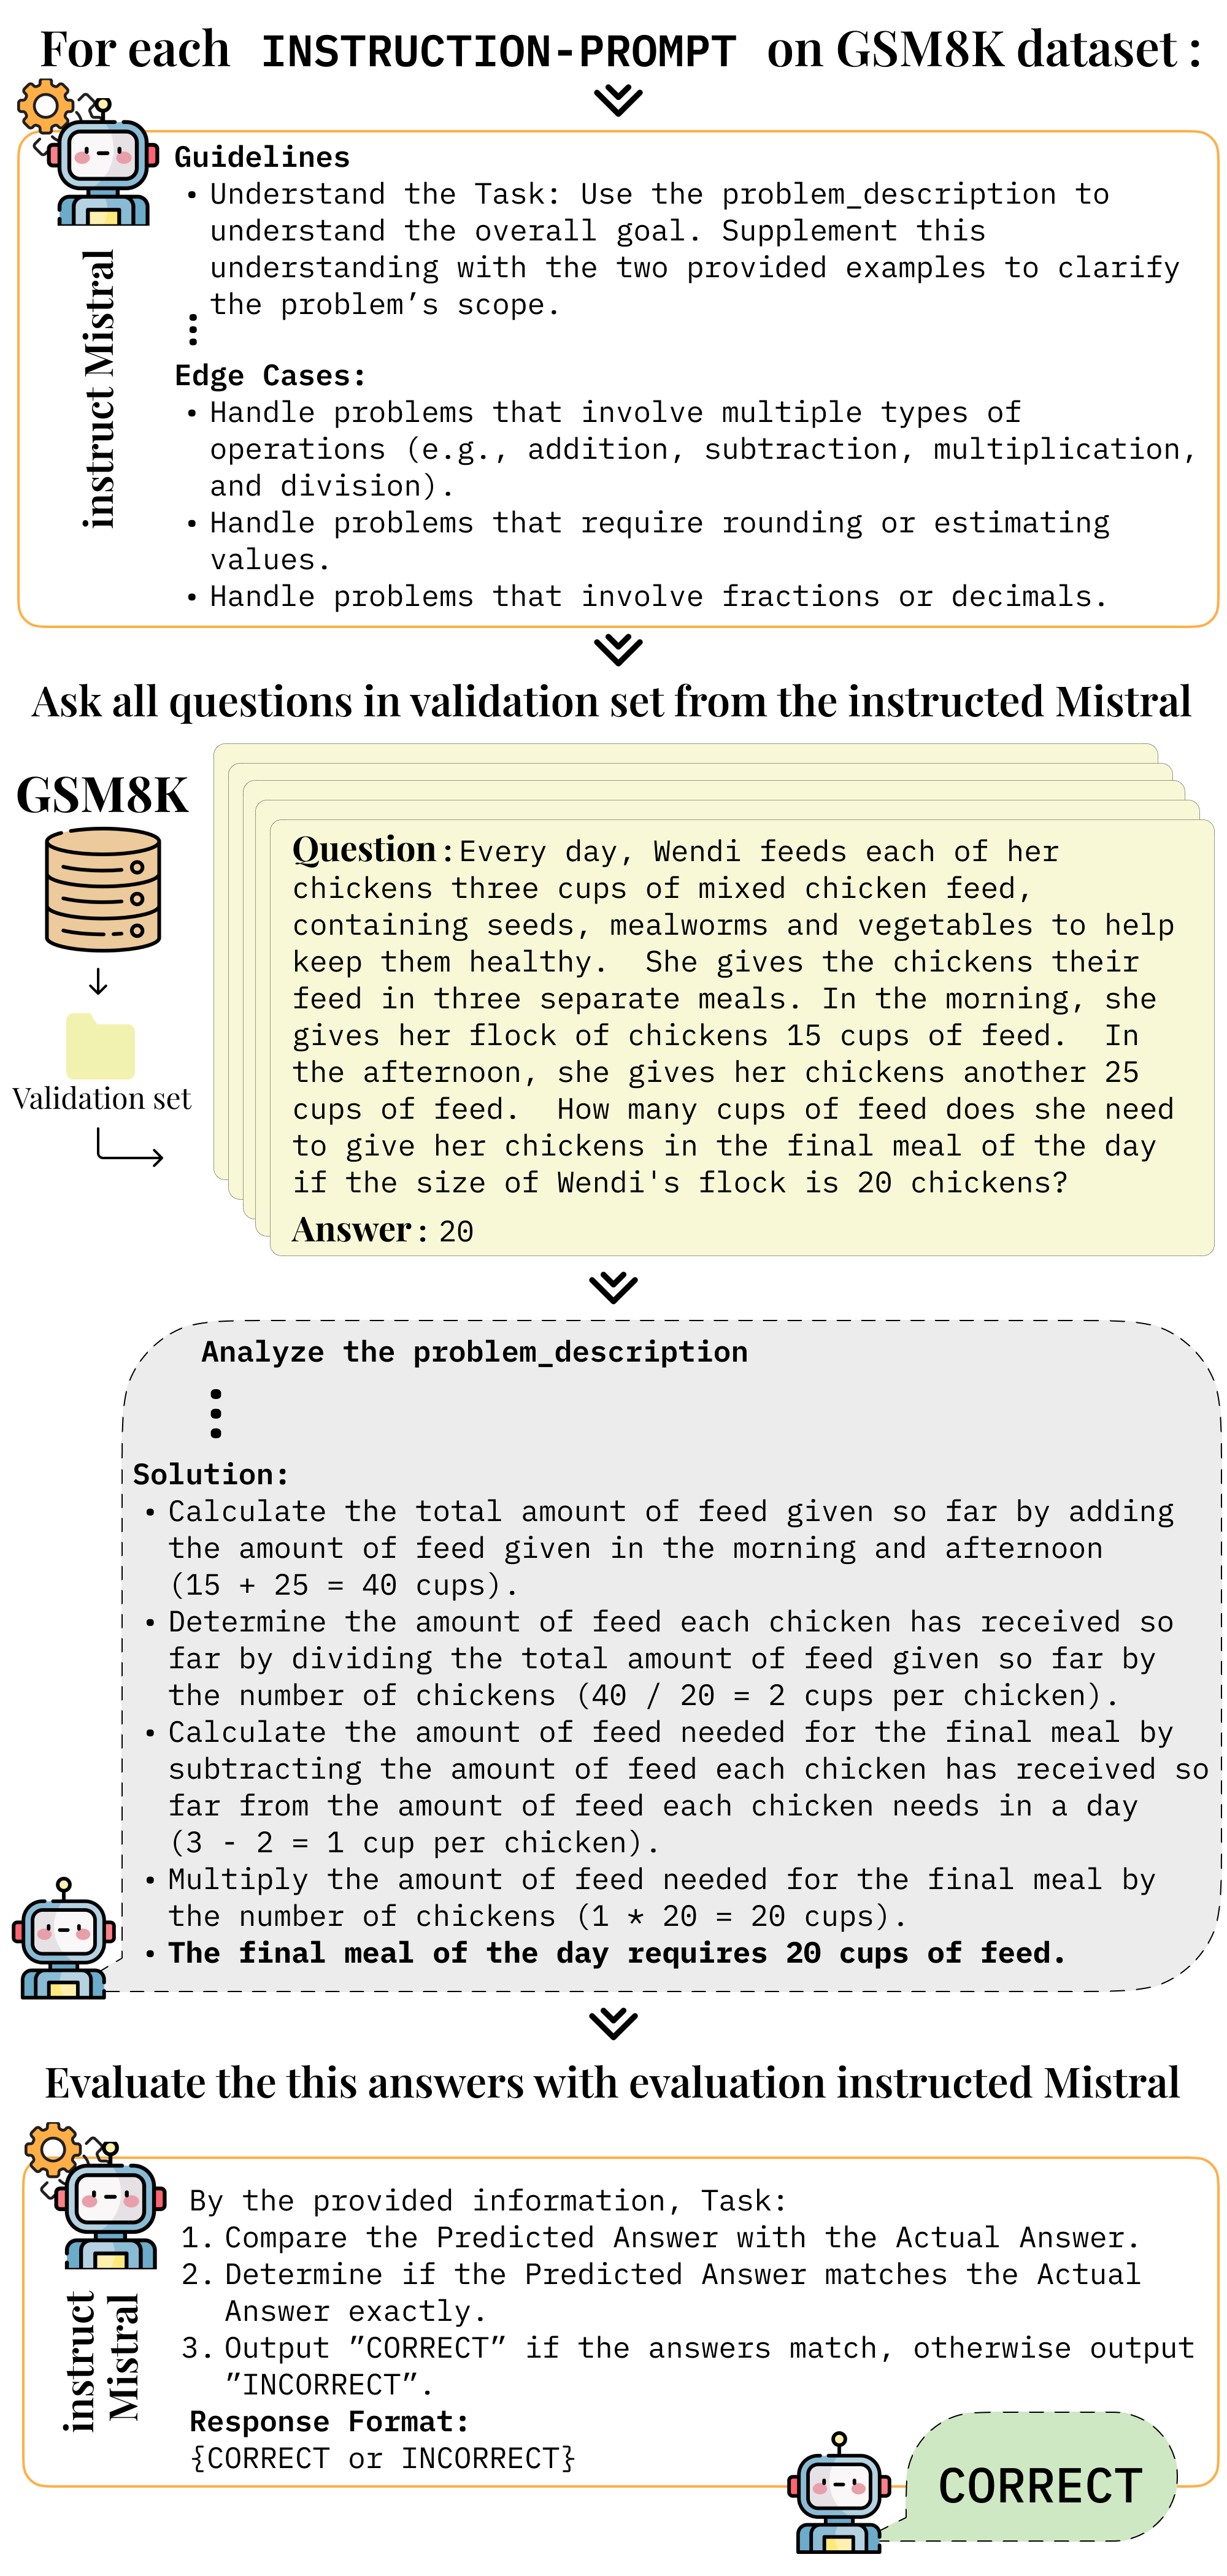
\includegraphics[width=90mm]{images/evaluation}
	\caption{دیاگرام مرحله ارزیابی روش مولد اعلان ساده}
	\label{fig_evaluation}
\end{figure}
























